\subsubsection{Synchronous vs. Asynchronous I/O}\label{subsubsec:sync}
%What is B/NB I/O?
I/O can be handled either synchronously or asynchronously. A synchronous I/O operation is blocking, i.e., the thread that executes the current job is in a waiting state, where it does not compute anything else, until it gets a response. An asynchronous I/O operation is non-blocking and therefore allows the thread to execute another job while waiting for the I/O operation to finish. This is illustrated on \Cref{fig:syncasync}. The figure does not show the overhead caused by using asynchronous I/O, which causes this to not be the best solution for all applications, especially if there are many short I/O operations \cite{ms-syn-asyn}.

\begin{figure}[H]
  \centering
  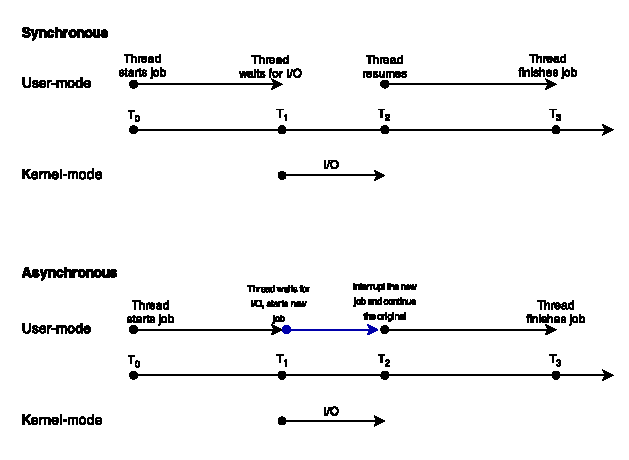
\includegraphics[scale=1.2]{billeder/sync-async.pdf}  
  \caption{Synchronous and asyncronous execution. Based on \cite{ms-syn-asyn}.}
  \label{fig:syncasync}
\end{figure}

This is the case for one or few users, but if there are many users at once they either have to wait in queue for previous I/O operations to finish, or each operation has to be executed in its own thread, which would potentially result in many active threads, requiring a lot of memory.  As pointed out by \citet{amir} it is worth noting that an asynchronous call that results in a synchronous operation causes the application to block, and therefore should be considered during implementation.

To allow the server to receive inputs from many clients at once, the client/server communication is implemented asynchronously. When the server receives an input, it is asynchronously sent to a dispatcher which sends it to the correct game thread; this is described in \Cref{sec:server}. Because of the many parts that have to interact, it is hard to determine if this implementation behaves as expected without testing it, but changing to a synchronous implementation would not be very expensive, as the asynchronous code is very similar to the synchronous code thanks to .NET's \texttt{Async} and \texttt{Await} keywords \cite{ms-asyn}. Some games may have different requirements in regards to client/server communication. Making both implementations available at the same time, letting the user choose which one to use, would be relatively easy to do. This, however, adds some extra complexity to the code, as changes in one implementation would require similar changes in the other. 
%What are the advantages and disadvantages?

%Which alternative(s) is/are there?

%Why did we make the choice we did?

%How flexible is it?
% - Could it easily be changed? 
% - Could both be implemented and the framework-user decides which one to use?
%
%\section{Synchronous vs. Asynchronous I/O}\fxfatal{This section will be rewritten with proper sources.}
%For the client/server socket communication, a choice between synchronous and asynchronous I/O has to be taken.
%% % blocking % %
%Synchronous I/O can have a better performance than asynchronous, but can cause problems when using a threaded architecture that spawns a new thread for each client. This is particularly true when the server should be scalable in regards to its number of connected clients. There might be 5 and there might be 5000 or even more.
%Tests show that threads are very efficient when it comes to memory and context switching, but only when the threads are kept alive for the entire execution of an application. This is not the case for our application, which will likely have many connections of varying durations during its up-time. \fixme{cite}\\\\
%% % non-blocking % %
%Asynchronous I/O is chosen for this project. It scales well when there are many clients, and the system should scale well with a potentially large number of clients. A notable advantage of asynchronous is that it limits the number of concurrent threads. The server asynchronously accepts a connection request from a client, and then starts an asynchronous worker thread to handle communication with the client. Meanwhile it continues to listen for new client connections.
%

%The ability to scale well does not come for free, however. Non-blocking I/O is not always as fast as blocking I/O and this can result in decreased performance. 
